\documentclass{deagle}
\title{Determining Optimal Food Truck Locations \\ \Large Evaluating Neighborhoods in Austin, Texas}
\begin{document}
\maketitle

%--------------------------------------------------------------------------------
%	INTRODUCTION
%--------------------------------------------------------------------------------

\section*{Introduction}

The audience for this data science problem will be owners and operators of traveling food trucks. As food truck operators enter a new city and a new market, a persistent question will be: where to park the foodtruck for maximum revenue. We will attempt to use data science and data from Foursquare to allow foodtruck operators to make a data-informed decision about where to park their food truck.

In this project we will determine the optimal Austin neighborhood to park a new food truck in. We will understand each Austin neighborhood's proximity to popular nightlife spots, as well as how saturated the food truck market is in the given neighborhood.

\section*{Data}

In order to solve this problem we will firstly need data on Austin neighborhoods. As no data set readily exists for Austin, Texas, we'll have to scrape Wikipedia for neighborhood information. \href{https://en.wikipedia.org/wiki/Category:Neighborhoods_in_Austin,_Texas}{This Wikipedia page} contains a list of Austin neighborhoods. Clicking a neighborhood shows that most pages have a \emph{Coordinates} section in the top-right which links to a \href{https://geohack.toolforge.org/geohack.php?pagename=Anderson_Mill,_Austin,_Texas&params=30_27_18_N_97_48_33_W_region:US-TX_type:city(8953)}{geohack page}.

Food trucks perform best in areas with a lot of nighlife spots. So we'll want to measure how many bars and nightlife spots are close to each neighborhood. We'll also want to measure how many foodtrucks are already in certain neighborhoods, to find neighborhoods that are less competitive. All of this data can be obtained through the \href{https://foursquare.com/developers/apps}{Foursquare API}.

Here is an example of using the Foursquare API in Python to retrieve nightlife spots near Austin, Texas. 

\begin{file}[use-foursquare.py]
\begin{lstlisting}[language=Python]
#! /usr/bin/python
import pandas as pd
import requests

def venues(latitude, longitude, category):
    """ Returns venues within a 1 km radius of a location """
    url = 'https://api.foursquare.com/v2/venues/explore?client_id={}' \
          '&client_secret={}&ll={},{}&v=20201120&categoryId={}' \
          '&radius=1000&limit=50'.format(client_id, client_secret, \
                                         latitude, longitude, category)
    results = requests.get(url).json()
    if results['meta']['code'] == '429':
        raise ValueError('Foursquare Quota Exceeded')
    return pd.json_normalize(results['response']['groups'][0]['items'])

df_nl = venues(30.3076863, -97.8934851, '4d4b7105d754a06376d81259')
\end{lstlisting}
\end{file}

And here is the resulting information:

\begin{ctable}{3}
    \textbf{Venue} & \textbf{Latitude} & \textbf{Longitude} \\ \hline
    The Common Interest & 30.366192 & -97.729144 \\ \hline
    Slick Willie's Family Pool & 30.366677 & -97.729049 \\ \hline
    Water 2 Wine & 30.362011 & -97.742086 \\ \hline
    Nosh \& Bevvy & 30.365414 & -97.728802 \\ \hline
    Buddy's & 30.368978 & -97.727205 \\ \hline
\end{ctable}

\section*{Methodology}

\subsection*{Overall Methodology}

Our overall methodology for this project will be to:

\begin{enumerate}
	\item Procure a list of neighborhoods in Austin, Texas
	\item Determine the number of nightlife spots in each neighborhood
	\item Determine the number of food trucks in each neighborhood
	\item Find the neighborhood with many bars and few food trucks
	\item Within that neighborhood, locate the largest cluster of bars
	\item Find the ideal parking spot as the midpoint of that cluster
\end{enumerate}

\subsection*{Procure a List of Neighborhoods in Austin, Texas}

As stated in the Data section, \href{https://en.wikipedia.org/wiki/Category:Neighborhoods_in_Austin,_Texas}{This Wikipedia page} has a list of Austin neighborhoods, each neighborhood having its own Wikipedia page. I found that the number of neighborhoods was low enough, and the pages differed enough, that a semi-manual process for procuring this list was ideal. For example, some of the Wikipedia pages listed coorindates in DD (decimal degrees) and some in DMS (degrees minutes seconds). I've created CSV file of Austin neighborhoods which can be found \href{https://github.com/bryandeagle/Coursera_Capstone/raw/main/data/austin.csv}{at this link}.

\subsection*{Determine the Number of Nightlife Spots}

Foursquare has a \emph{Nightlife} category. The challenge with using that broad category is that it includes things like hotel bars and sports bars, which typically also serve food. So to get the most accurate results, we'll select the subcategories of \emph{Nightlife} that don't likely serve food.

These are: \emph{Beach Bar}, \emph{Beer Bar}, \emph{Beer Garden}, \emph{Champagne Bar}, \emph{Cocktail bar}, \emph{Dive Bar}, \emph{Gay Bar}, \emph{Hookah Bar}, \emph{Karaoke Bar}, \emph{Pub}, \emph{Sake Bar}, \emph{Speakeasy}, \emph{Tiki Bar}, \emph{Whisky Bar}, \emph{Wine Bar}, \emph{Brewery}, \emph{Lounge}, \emph{Nightclub}, and \emph{Other Nightlife}.

We'll use the \href{https://developer.foursquare.com/docs/api-reference/venues/explore/}{Explore API Endpoint} in Foursquare and set the limit to 50 (max) and the radius to 1 km.

\subsection*{Determine the Number of Food Trucks}

Foursquare has a \emph{Food Truck} category we can use to enumerate food trucks in a given neighborhood. Similar to nightlife, we'll use the \href{https://developer.foursquare.com/docs/api-reference/venues/explore/}{Explore API Endpoint} in Foursquare and set the limit to 50 (max) and the radius to 1 km.

\subsection*{Find the Neighborhood with Many Bars and Few Foodtrucks}

To accomplish this, we'll create a new index, called the \emph{Foodtruck-to-Nightlife Ratio (FNR)}. The formula for this ratio will be:

% Math equation/formula
\begin{equation}
	FNR = \frac{N_{foodtrucks}}{N_{nightlife}}
\end{equation}

As you can tell from the formula, the number of nightlife spots cannot be zero, or this ratio cannot be calculated. Actually we'll want to avoid neighborhoods with too few nightlife spots, so we'll create a threshold below which we won't consider the neighborhood. I've set this threshold at \emph{five} nightlife spots for this project.

\subsection*{Within that Neighborhood, Find the Largest Cluster of Bars}

We'll use the \emph{DBSCAN (Density-based spatial clustering of applications with noise)} method for creating clusters. Benefits of using DBSCAN are that we don't have to know how many clusters to create, and it will properly reject noise -- bars that are not close to any other bars.

\subsection*{Find the Ideal Parking Spot as the Midpoint of that Cluster}

Once we've identified our cluster of bars to target, we'll average the latitudes and longitudes of those bars, to find the ideal place to park our food truck. Then we'll convert that latitude-longitude-pair into a street address.

\section*{Results}

\subsection*{Enumerating Neighborhoods}

After getting the list of Austin neighborhoods, and using Foursquare to read the number of nightlife spots and the number of food trucks in each location, the Foodtruck-to-Nightlife Ratio was able to be calculated. After removing the neighborhoods with less than five bars, our results were as follows:

\begin{center}
\begin{tabular}{|c|c|c|c|c|c|} \hline
    \textbf{Neighborhood} & \textbf{Latitude} & \textbf{Longitude} & \textbf{Nightlife} & \textbf{Food Truck} & \textbf{FNR} \\ \hline
    North Shoal Creek     & 30.365300 & -97.733500 & 8          & 3          &  0.375000 \\ \hline
    Clarksville           & 30.280833 & -97.762222 & 5          & 2          &  0.400000 \\ \hline
    Saint John            & 30.330000 & -97.698000 & 6          & 3          &  0.500000 \\ \hline
    Bremond Block         & 30.270556 & -97.746389 & 158        & 117        &  0.740506 \\ \hline
    Downtown Austin       & 30.271000 & -97.743000 & 169        & 130        &  0.769231 \\ \hline
    Mueller Community     & 30.289444 & -97.702636 & 7          & 6          &  0.857143 \\ \hline
    Congress Avenue       & 30.267778 & -97.742500 & 182        & 163        &  0.895604 \\ \hline
    Zilker                & 30.250000 & -97.766667 & 15         & 16         &  1.066667 \\ \hline
    Travis Heights        & 30.241667 & -97.741667 & 5          & 7          &  1.400000 \\ \hline
    Rainey Street         & 30.259444 & -97.738333 & 120        & 177        &  1.475000 \\ \hline
    North Burnet–Gateway  & 30.393000 & -97.721000 & 9          & 14         &  1.555556 \\ \hline
    Blackland             & 30.280991 & -97.722097 & 6          & 11         &  1.833333 \\ \hline
    Willow–Spence Streets & 30.259167 & -97.734444 & 82         & 174        &  2.121951 \\ \hline
    Swedish Hill          & 30.275000 & -97.729444 & 14         & 38         &  2.714286 \\ \hline
    Bouldin Creek         & 30.249344 & -97.755253 & 10         & 60         & 6.000000 \\ \hline
    South Congress        & 30.250000 & -97.750000 & 9          & 54         &  6.000000 \\ \hline
\end{tabular}
\end{center}

\subsection*{Determining the Best Neighborhood}

The bar chart below shows the Foodtruck-to-Nightlife ratio of Austin neighborhoods. As we can see, \textbf{North Shoal Creek} has the lowest ratio. There are, however, other neighborhoods with similar ratios, in case we find an issue with North Shoal Creek.

\begin{center}
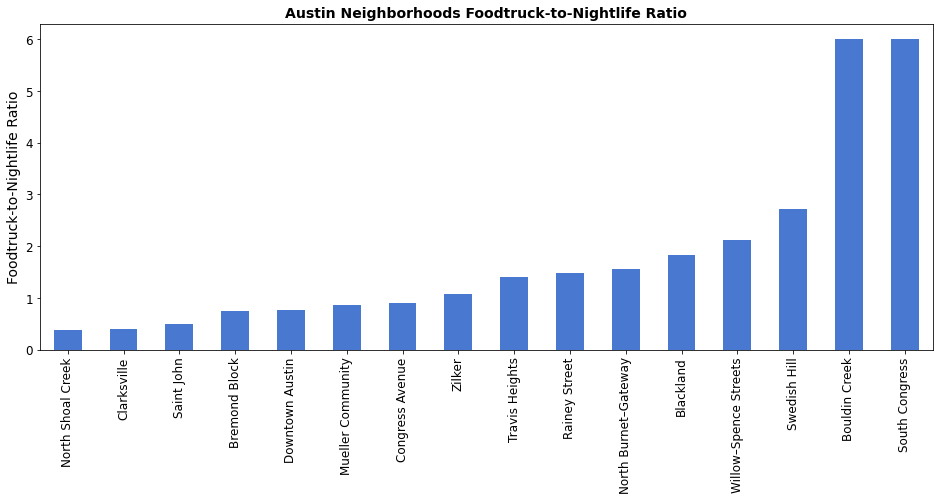
\includegraphics[scale=0.45]{bar}
\end{center}

\subsection*{Finding the Best Parking Spot in the Neighborhood}

We use the \emph{DBSCAN} method to put the nightlife spots into clusters, and filter out the noise. As we can see from the map below, there are several "loner" nightlife spots (shown in black), but a definite cluster of bars off of Burnet Road (shown in pink).

Our ideal parking location is the average of the cluster of bars, and is shown by the green dot on the map. We use geopy to determine the address of that location is \textbf{8524, Burnet Road, Wooten, Austin, Travis County, Texas, 78757, United States of America}.

\begin{center}
    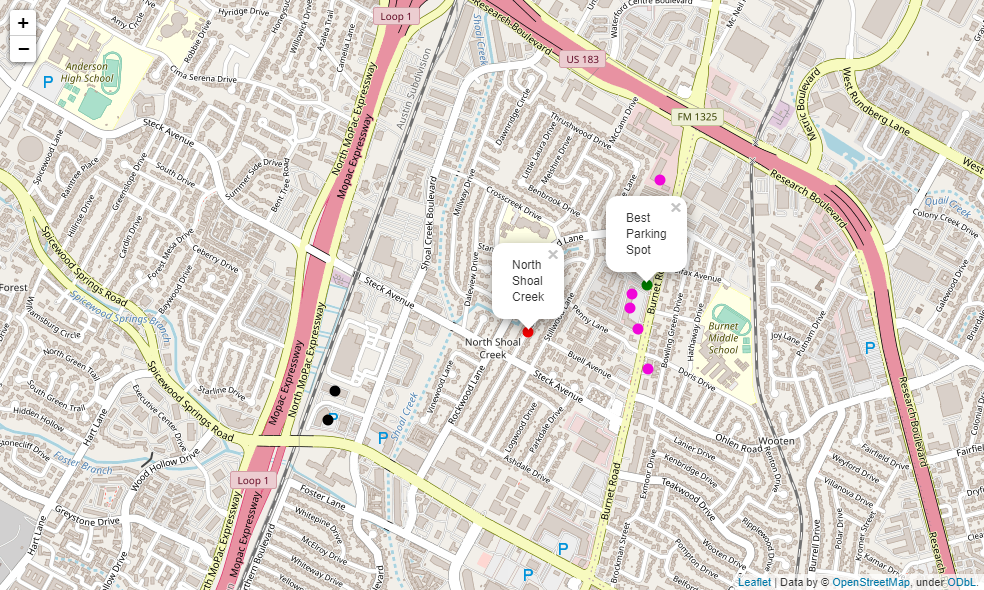
\includegraphics[scale=0.55]{map}
\end{center}

\section*{Discussion}

Overall, it appears the \emph{Foodtruck-to-Bar} ratio is a compelling metric for making a data-informed decision about where to park a new food truck. It also appears the DBSCAN clustering method was successful in finding clusters of nearby bars while rejecting loner bars.

\section*{Conclusion}

In conclusion, \textbf{North Shoal Creek} will be the best neighborhood to park our food truck in Austin, Texas. The ideal parking space in North Shoal Creek will be \textbf{8524, Burnet Road, Wooten, Austin, Travis County, Texas, 78757, United States of America}.

\end{document}